%% LyX 2.2.3 created this file.  For more info, see http://www.lyx.org/.
%% Do not edit unless you really know what you are doing.
\documentclass[english]{article}
\usepackage[T1]{fontenc}
\usepackage[latin9]{inputenc}
\usepackage{amsmath}
\usepackage{graphicx}
\usepackage{babel}
\begin{document}

\title{PHYS 7810: Practicum 1}

\author{Omkar H. Ramachandran}
\maketitle

\section*{Derivation of the core equation}

The Crank-Nicolson method works by equally sampling the forward euler
method at a given point $n$ and the backward euler scheme at $n+1$.
In essence, we end up using the value of $f\left(x_{mid}\right)$
where $x_{mid}$ is at the 'midpoint' between $x_{n}$ and $x_{n+1}$.
For the simple harmonic oscillator, we have the following two differential
equations:
\[
\dot{v}=-\omega_{0}^{2}x
\]
\[
\dot{x}=v
\]
Sampling $v$ at the midpoint between $n$ and $n+1$ yeilds the following:
\[
x_{n+1}-x_{n}=\frac{h}{2}\left(v_{n+1}+v_{n}\right)
\]
Where $h$ is the step size. Similarly, for $v$, we have
\[
v_{n+1}=v_{n}+hf\left(\frac{x_{n+1}+x_{n}}{2}\right)=v_{n}+hf\left(x_{n}+\frac{h}{4}\left[v_{n+1}+v_{n}\right]\right)
\]
where $f\left(x\right)=-\omega_{0}^{2}x$. It makes sense to solve
for $v_{n+1}$first, since it only depends on $x_{n}$ and $v_{n}$.
In essence,
\[
v_{n+1}=v_{n}-h\omega_{0}^{2}\left(x_{n}+\frac{h}{4}\left[v_{n+1}+v_{n}\right]\right)
\]
\[
\implies v_{n+1}\left[1+\frac{\omega_{0}^{2}h^{2}}{4}\right]=v_{n}\left[1-\frac{\omega_{0}^{2}h^{2}}{4}\right]-h\omega_{0}^{2}x_{n}
\]
Thus,
\[
v_{n+1}=\frac{v_{n}\left[1-\frac{\omega_{0}^{2}h^{2}}{4}\right]-h\omega_{0}^{2}x_{n}}{1+\frac{\omega_{0}^{2}h^{2}}{4}}
\]
Once $v_{n+1}$ is known, we can simply plug it into the $x$ equation
to get 
\[
x_{n+1}=x_{n}+\frac{h}{2}\left(v_{n+1}+v_{n}\right)
\]
thus giving us $x$ and $v$ for each time step

\subsection*{Additional optimizations made}
\begin{itemize}
\item Since floating point multiplication is much faster than floating point
division, the divisor in the $v$ equation, $1/\left(1+\frac{\omega_{0}^{2}h^{2}}{4}\right)$
was computed seperately outside the loop and at each timestep, this
variable 'pdt2om2' in crank\_nicolson.py was multiplied with the the
numerator.
\end{itemize}

\section*{Zero Crossing Loop}

To measure the zero crossing of the solution, $x\left[i\right]$ was
looped over $i$ till the sign of $x$ changed. If this condition
turned out to be true, the time of the zero crossing was taken to
be the midpoint of the line connecting $x\left[i\right]$ and $x\left[i-1\right]$
as follows:
\[
t_{cross}=t\left[i-1\right]+\frac{t\left[i\right]-t\left[i-1\right]}{\left|x\left[i\right]-x\left[i-1\right]\right|}\left(x\left[i-1\right]\right)
\]
The absolute value is simply so that we can treat $x\left[i\right]>x\left[i-1\right]$
and $x\left[i-1\right]>x\left[i\right]$ the same, thus removing one
extra if condition. We do not need to do this for $t\left[i\right]-t\left[i-1\right]$
since $t$ always increases.

\subsection*{Results of the Zero-Crossing measurement}

\begin{figure}
\begin{centering}
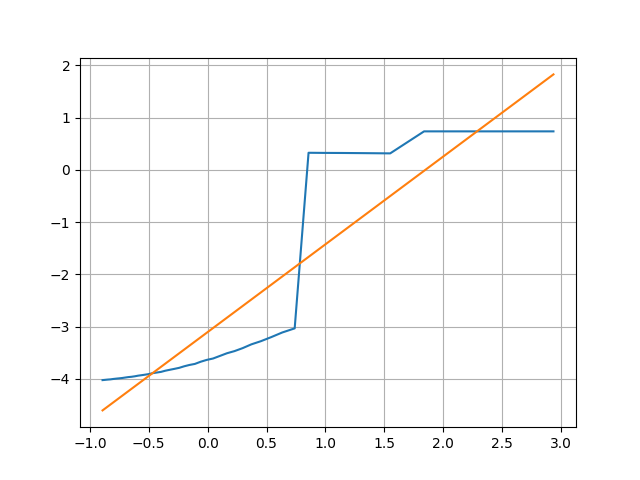
\includegraphics[scale=0.4]{freqplot}
\par\end{centering}
\caption{Zero crossing measurement done for between 2 and 45 points between
0 and $6\pi$. The $x$ axis of the log-log plot is the step size
while the $y$ axis is the error in the frequency $\left|f_{measured}-\omega_{0}/2\pi\right|$}
\end{figure}
For the chart obtained in figure $1$, the least squares fit was the
following: $x=1.6802t-3.1057$. However, as the number of data points
increased, the error in frequency stabilized at $\ln\left|f_{error}\right|\sim-4.1$,
suggesting that we're now hitting the limit of either the interpolation
in the zero-crossing measurement or the true limit of the method,
$O\left(\left(dt\right)^{2}\right)$. To verify this, the least squares
line for the frequency plot was obtained exclusively with coarser
grids and the tapering limit appeared to be $m_{lsq}\sim2$, suggesting
that this was indeed the frequency error of the method $O\left(\left(dt\right)^{2}\right)$.
A better way to verify this would be to interpolate with three points
to find the zero crossing and see if this limit is preserved.
\end{document}
